% ==================================================
% Section 3
% ==================================================
\section{Nominal Controller Simulation}

In this section, the nominal controller is simulated under the assumption that all model parameters are known. Therefore, the true parameter vector \(\theta\) is used directly in the control law.

\subsection{Simulation Parameters}

The plant parameters used in the simulation are selected as:
\begin{equation}
a_1=2,\quad
a_2=3,\quad
a_3=1,\quad
b_1=0.05,\quad
b_2=0.1,\quad
b_3=1.5,\quad
c=1.
\end{equation}

\noindent The reference model is chosen using a dominant second-order pair with an additional fast real pole:
\begin{equation}
\left(s^2+2\zeta\omega_n s+\omega_n^2\right)(s+p_3)
\end{equation}

where
\begin{equation}
\zeta=0.7,\qquad
\omega_n=2,\qquad
p_3=10\zeta\omega_n=14.
\end{equation}

\noindent Therefore:
\begin{equation}
\left(s^2+2.8s+4\right)(s+14)
=
s^3+16.8s^2+43.2s+56.
\end{equation}

\noindent Thus, the reference model parameters are:
\begin{equation}
\alpha_2=16.8,\qquad
\alpha_1=43.2,\qquad
\alpha_0=56.
\end{equation}

\noindent And the reference model polynomial is:
\begin{equation}
s^3+16.8s^2+43.2s+56.
\end{equation}

\noindent For a third-order polynomial
$s^3+a s^2+b s+c$,
the Routh--Hurwitz stability conditions are:
\begin{equation}
a>0,\qquad b>0,\qquad c>0,\qquad ab>c.
\end{equation}

\noindent In this case:

\begin{equation}
16.8>0,\qquad
43.2>0,\qquad
56>0,
\end{equation}

and
\begin{equation}
16.8\cdot43.2
=
725.76
>
56.
\end{equation}

\noindent Therefore, the reference model is stable according to the Routh--Hurwitz criterion.

\noindent The controller parameters are selected as:
\begin{equation}
\lambda_1=4,\qquad
\lambda_2=4,\qquad
k_z=5.
\end{equation}

\noindent The corresponding error-filter polynomial is:
\begin{equation}
s^2+4s+4=(s+2)^2
\end{equation}

\noindent which is stable. The reference input is chosen as a constant angular setpoint:
\begin{equation}
r(t)=\frac{\pi}{4}\;\mathrm{rad}\quad(45^\circ),
\end{equation}
representing a step command for the manipulator to reach and hold a fixed angle.

\subsection{Simulation Results}

The simulation results are presented in figures~\ref{fig:nominal_tracking_and_control} and~\ref{fig:nominal_errors}. The plant output follows the reference model output to the target angle, and the tracking error remains close to zero throughout the transient and steady state. The filtered error stays at the numerical floor of the integrator, which is consistent with the theoretical prediction that, under exact parameter knowledge and matched initial conditions, \(z(t)\) is identically zero.

\begin{figure}[H]
    \centering
    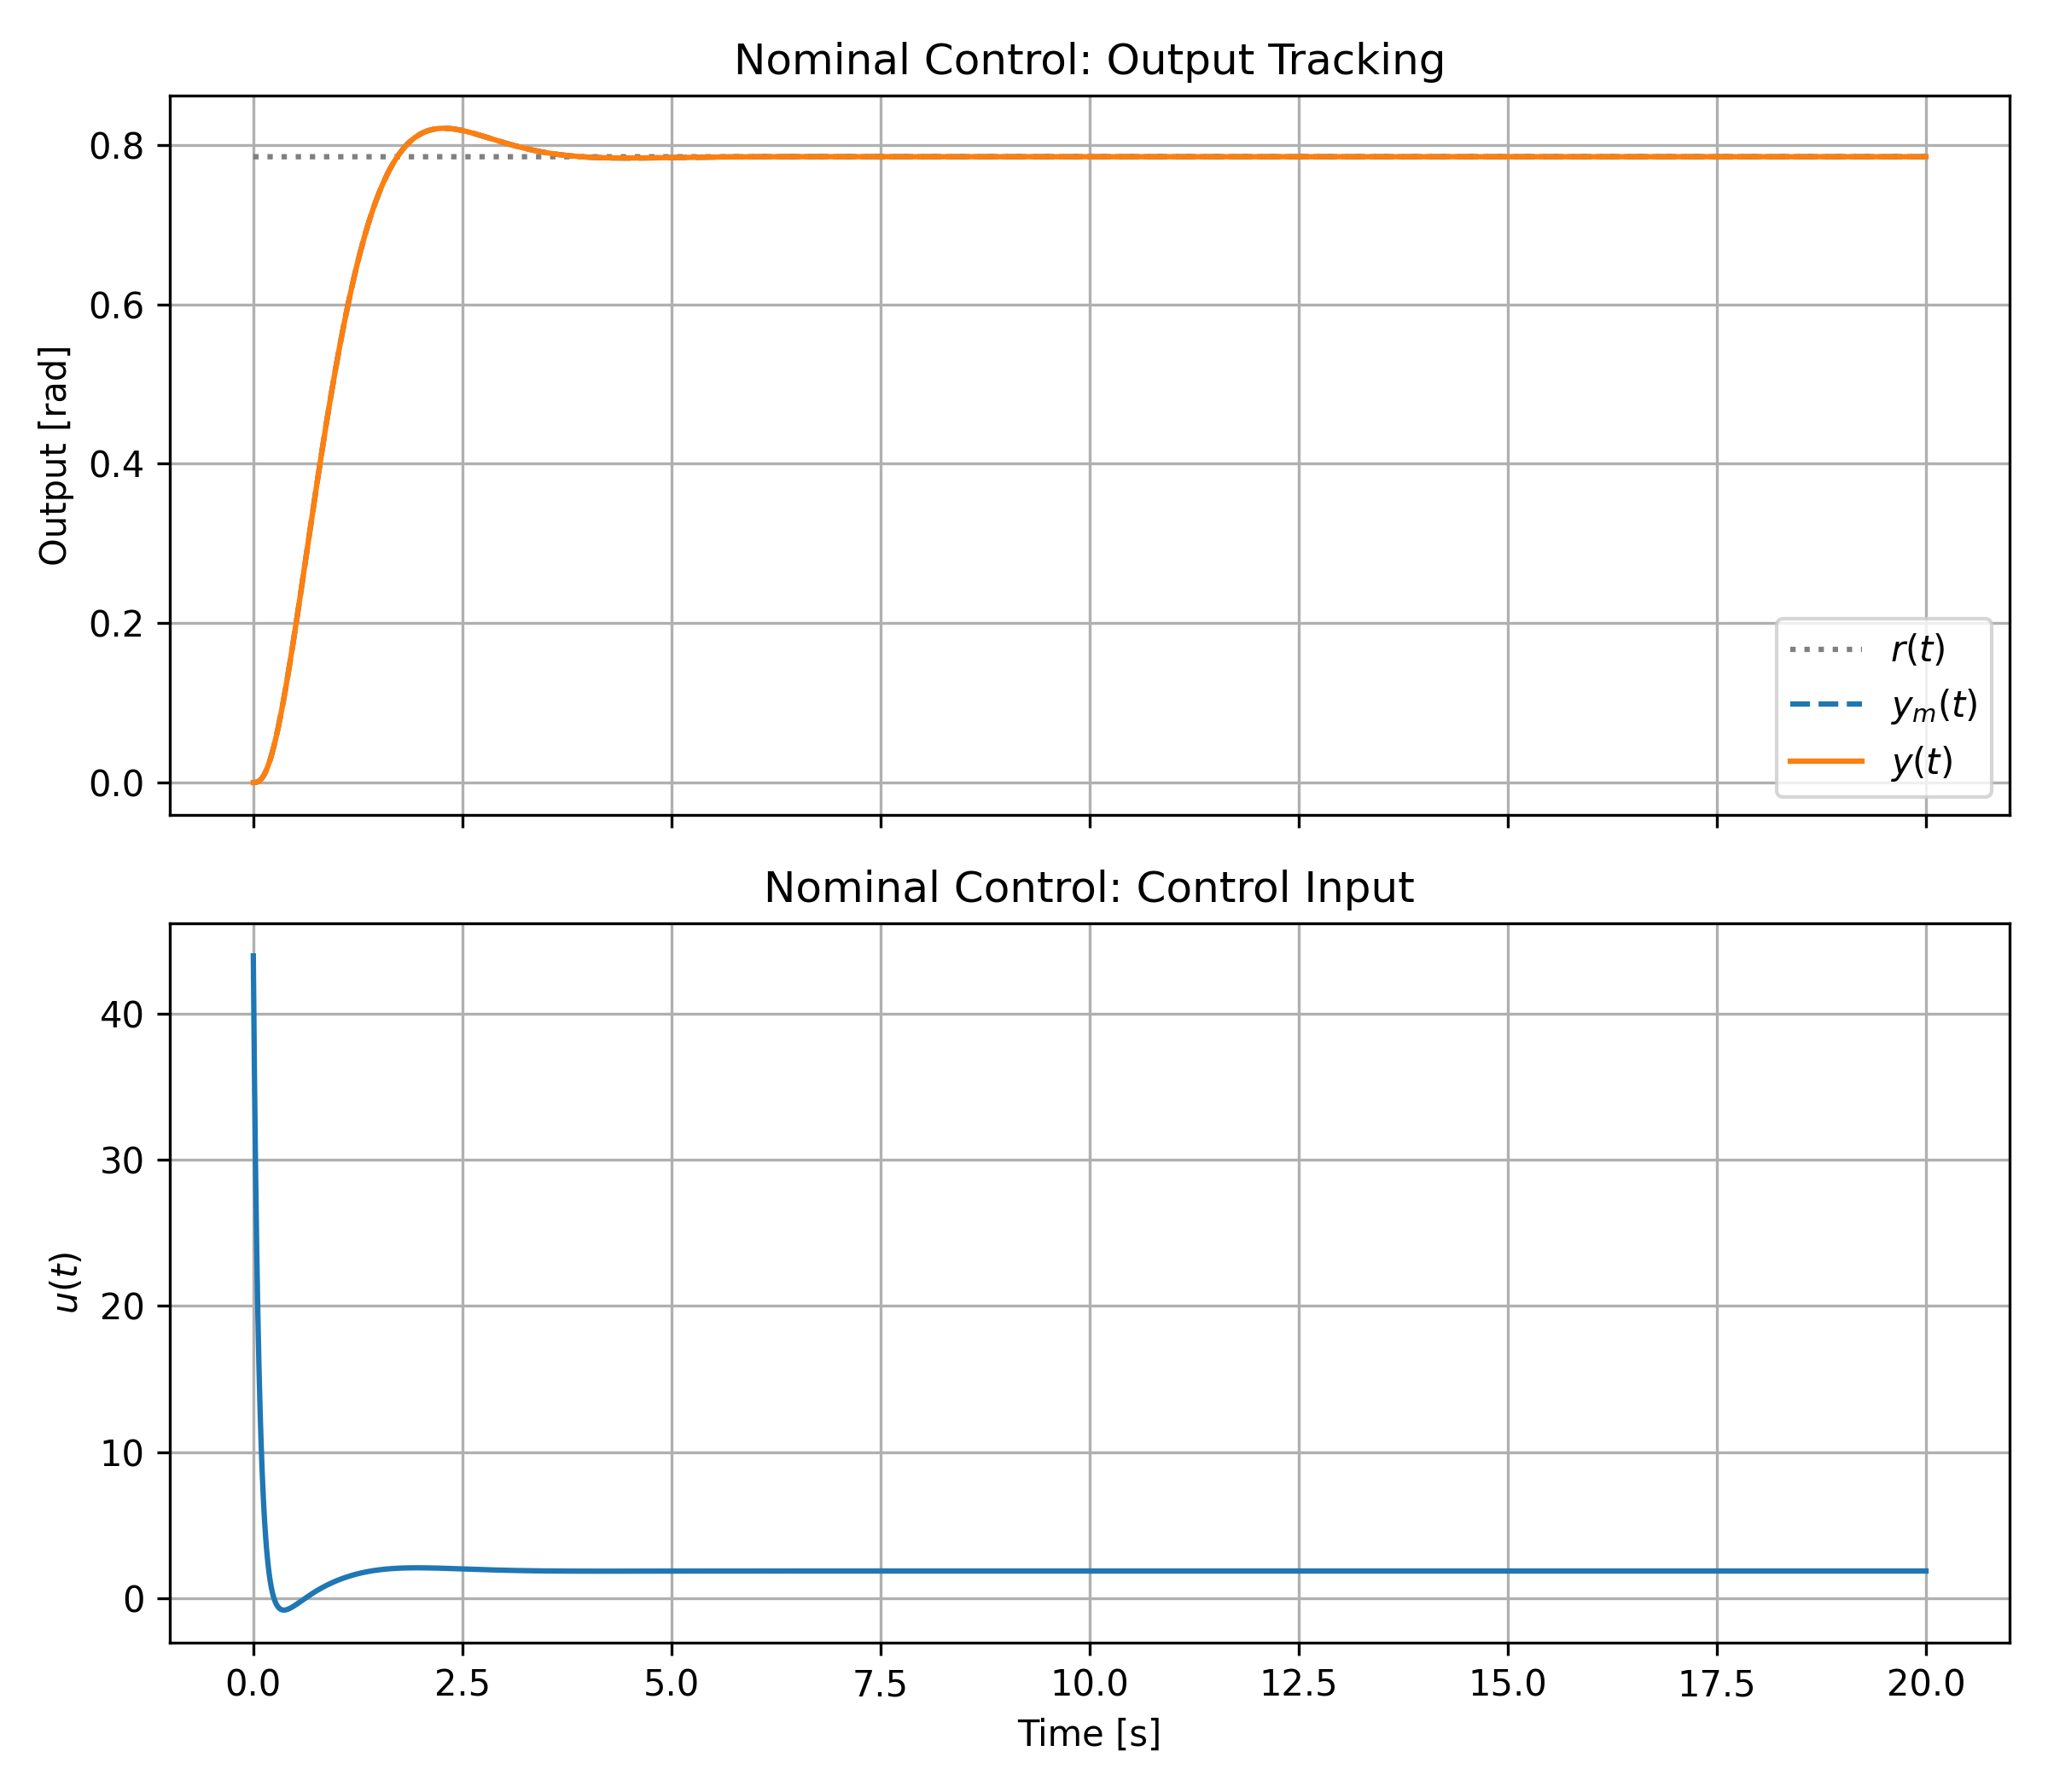
\includegraphics[width=0.6\textwidth]{figs/hw/nominal_tracking_and_control.png}
    \caption{Reference command \(r(t)\), reference model output \(y_m(t)\), and plant output \(y(t)\) (top); Control input \(u(t)\) (bottom).}
    \label{fig:nominal_tracking_and_control}
\end{figure}

\begin{figure}[H]
    \centering
    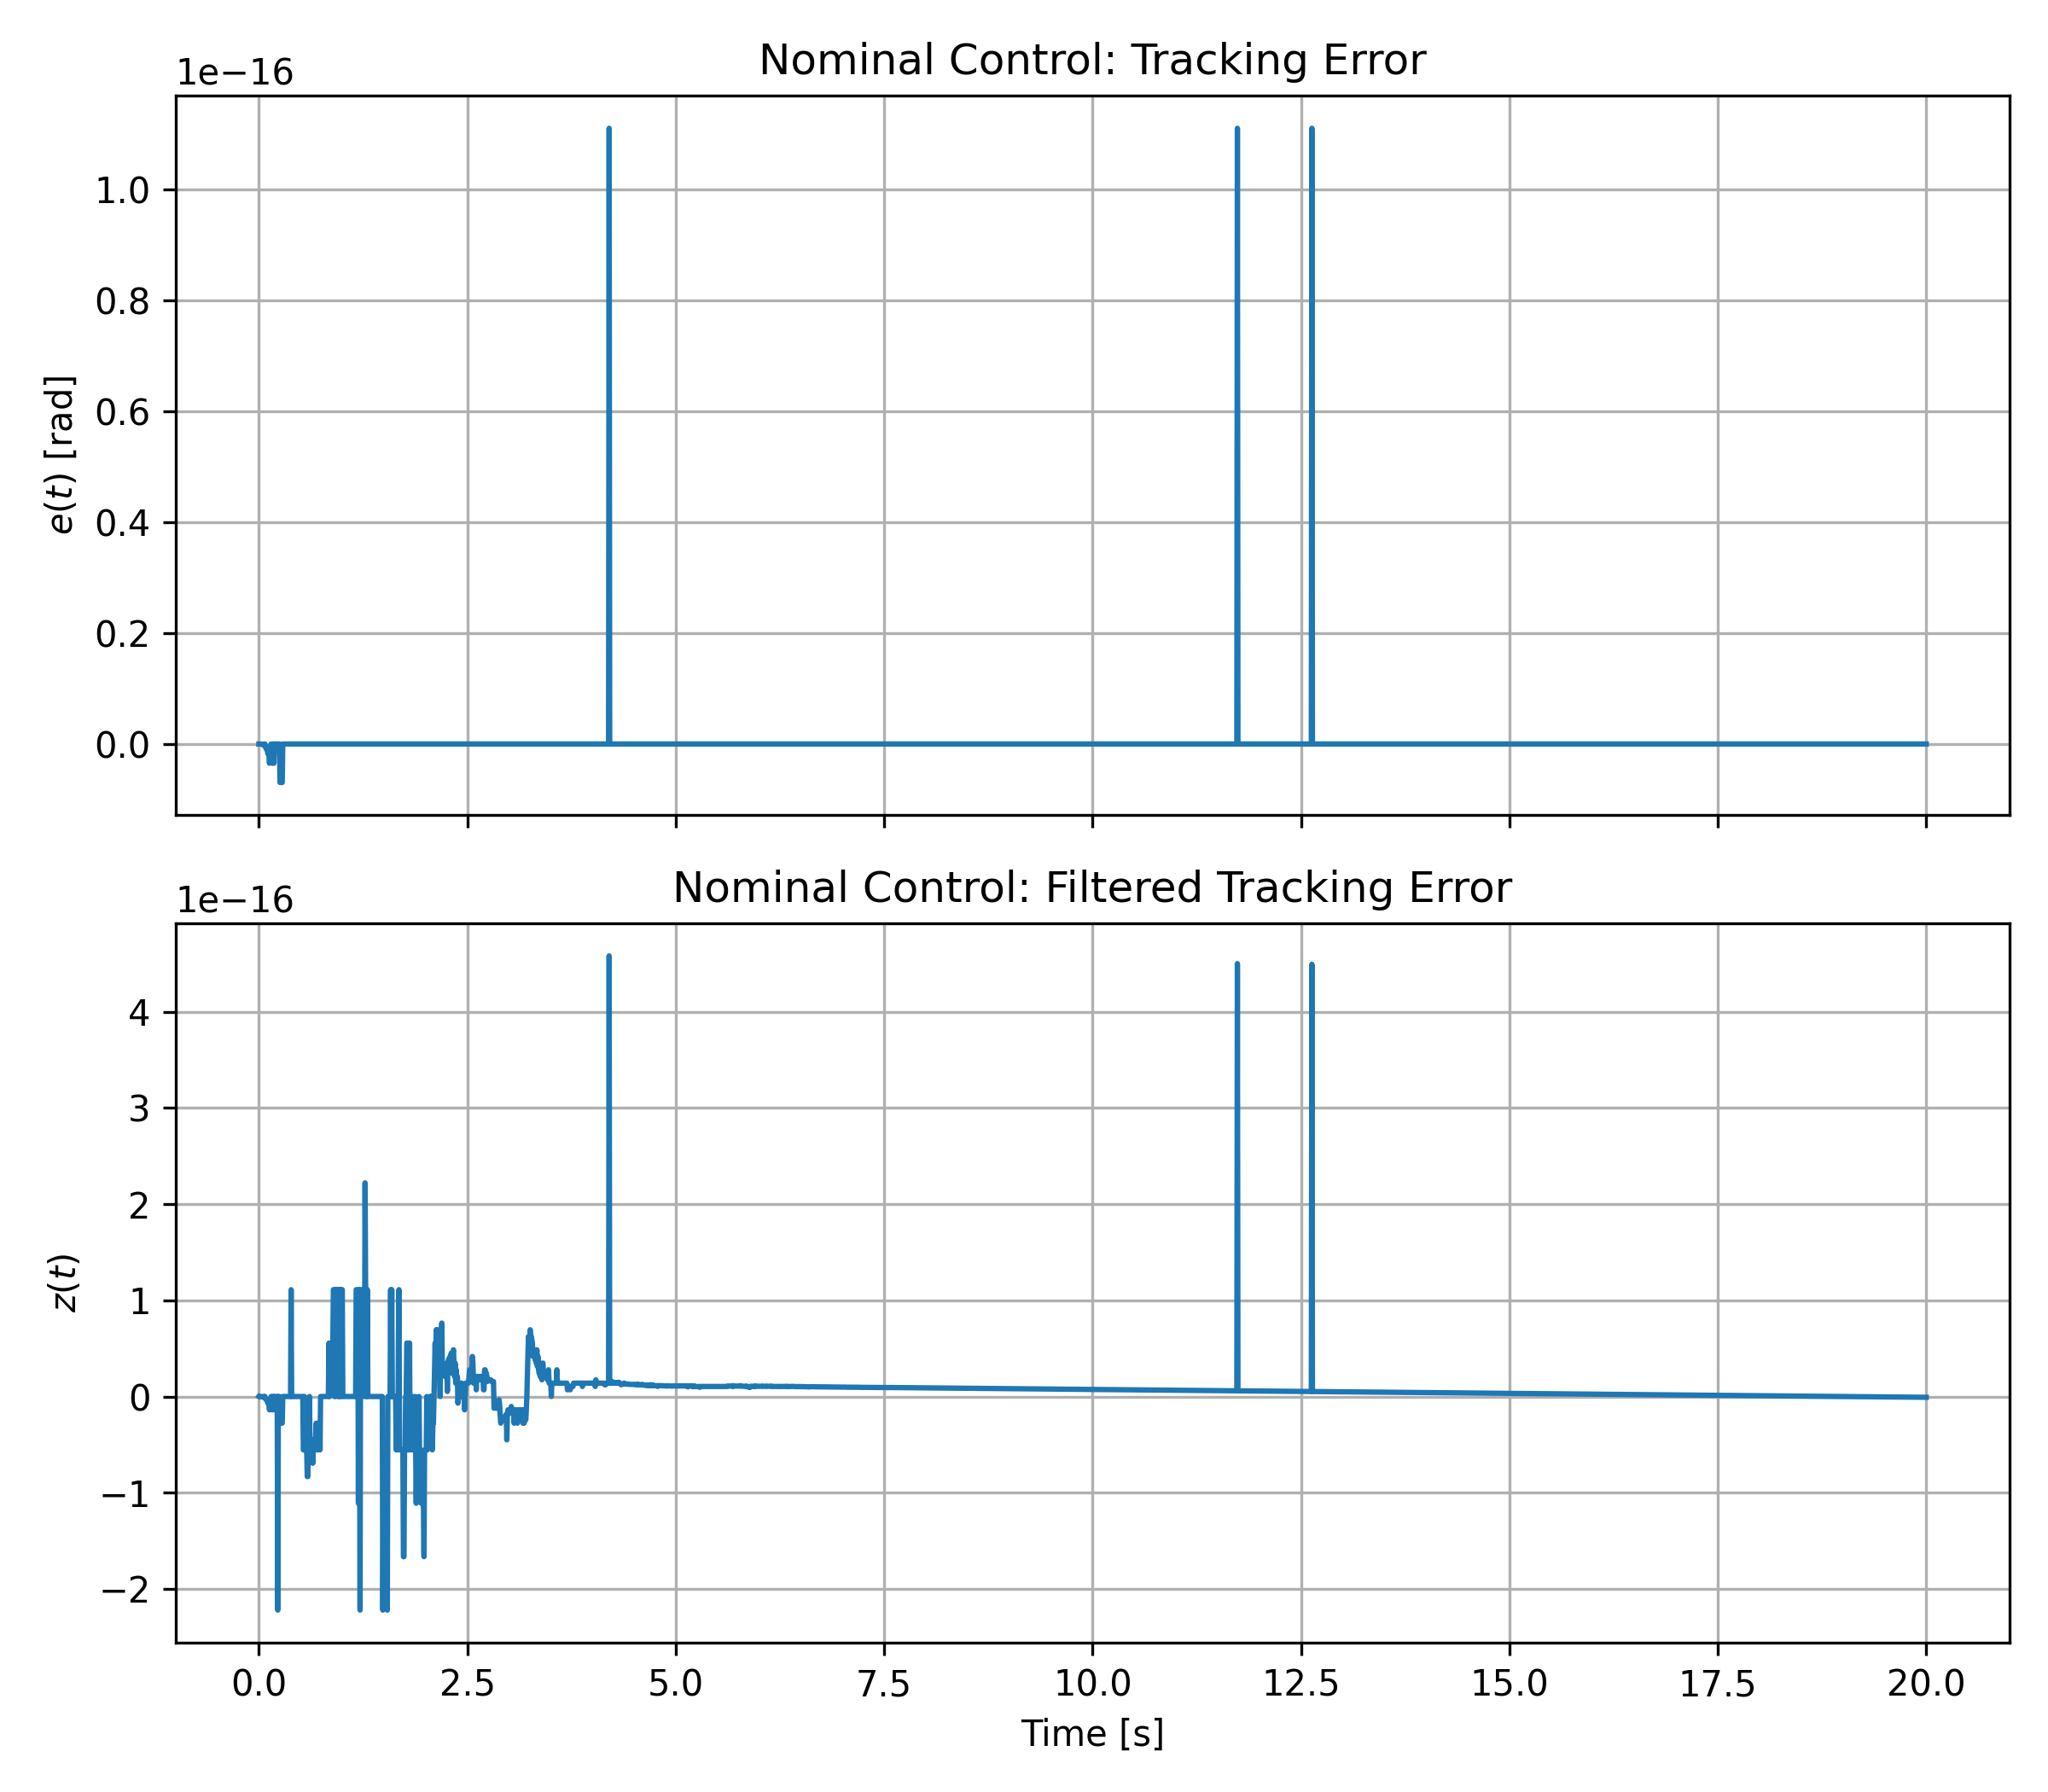
\includegraphics[width=0.6\textwidth]{figs/hw/nominal_errors.png}
    \caption{Tracking error \(e(t)=y(t)-y_m(t)\) (top); Filtered tracking error \(z(t)=\ddot{e}+\lambda_2\dot{e}+\lambda_1 e\) (bottom).}
    \label{fig:nominal_errors}
\end{figure}

\noindent The simulation validates the nominal controller derived in Section 2. Since all plant parameters are assumed to be known, the controller can fully compensate for the nonlinear plant dynamics. As a result, the tracking error converges to zero and the plant output closely follows the reference model output. Any small residual error observed in the simulation is caused by numerical integration errors rather than by the controller itself. These results provide a baseline for comparison with the adaptive controller presented in the next section, where the plant parameters are assumed to be unknown.

\bigskip
